\documentclass[11pt, convert={outext=.png}]{standalone}
\usepackage{tikz}
\usetikzlibrary{math}
\usepgflibrary{patterns.meta}
\usetikzlibrary{patterns.meta}

\begin{document}
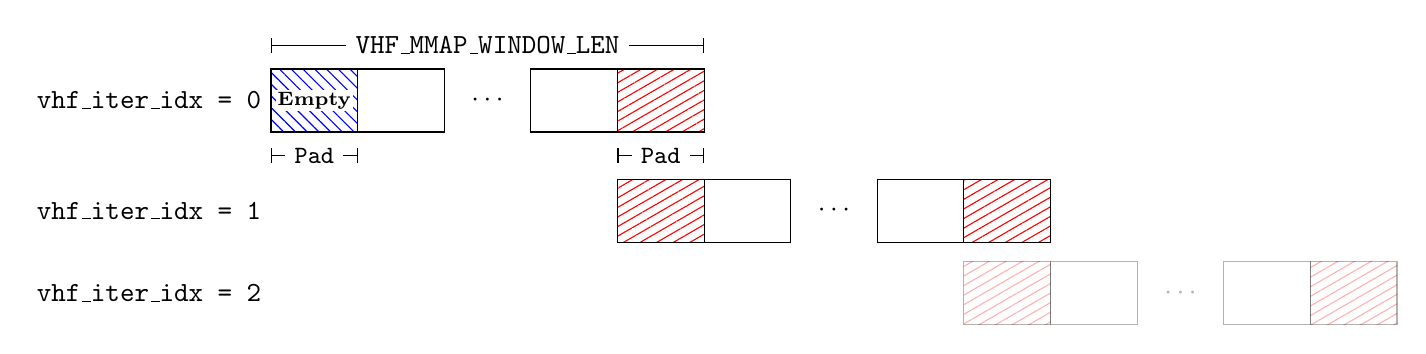
\begin{tikzpicture}
	% Constants
	\tikzmath{\pagewidth = 1.1; \pageheight=0.8; \textstagger=-0.30;}

	\begin{scope}
		\node[anchor=east] at (0, \pageheight/2) {\texttt{vhf\_iter\_idx = 0}};

		% Pages
		\draw[pattern={Lines[angle=-45,distance={3pt}]},pattern color=blue] (0,0) rectangle +(\pagewidth,\pageheight)
		node [anchor=center, fill=white, inner sep=0.7pt, outer sep=0.7pt] at (\pagewidth/2, \pageheight/2) {\scriptsize \textbf{Empty}};
		\draw (\pagewidth,0) rectangle ++(\pagewidth,\pageheight)
		++(0,-\pageheight) node[anchor=center] at (2.5 * \pagewidth, \pageheight/2) {$\cdots$} ++(\pagewidth,\pageheight)
		++(0,-\pageheight) rectangle ++(\pagewidth,\pageheight);
		\draw[pattern={Lines[angle=30,distance={3pt}]},pattern color=red] (4*\pagewidth,0) rectangle +(\pagewidth,\pageheight);

		% Labels
		\draw[|-|] (0, \pageheight - \textstagger) -- ++(5*\pagewidth, 0) node[midway,fill=white] {\texttt{VHF\_MMAP\_WINDOW\_LEN}};
		\draw[|-|] (0, \textstagger) -- ++(\pagewidth, 0) node[midway,fill=white] {\small\texttt{Pad}};
		\draw[|-|] (4*\pagewidth, \textstagger) -- ++(\pagewidth, 0) node[midway,fill=white] {\small\texttt{Pad}};
	\end{scope}

	% Cascading subsequent windows
	\begin{scope}[shift={(0,2.0*\textstagger-\pageheight)}]
		\node[anchor=east] at (0, \pageheight/2) {\texttt{vhf\_iter\_idx = 1}};

		\begin{scope}[shift={(4*\pagewidth,0)}]
			% Pages
			\draw[pattern={Lines[angle=30,distance={3pt}]},pattern color=red] (0,0)  rectangle +(\pagewidth,\pageheight);
			\draw (\pagewidth,0) rectangle ++(\pagewidth,\pageheight)
			++(0,-\pageheight) node[anchor=center] at (2.5 * \pagewidth, \pageheight/2) {$\cdots$} ++(\pagewidth,\pageheight)
			++(0,-\pageheight) rectangle ++(\pagewidth,\pageheight);
			\draw[pattern={Lines[angle=30,distance={3pt}]},pattern color=red] (4*\pagewidth,0) rectangle +(\pagewidth,\pageheight);
		\end{scope}
	\end{scope}
	\begin{scope}[shift={(0,5.5*\textstagger-\pageheight)}]
		\node[anchor=east] at (0, \pageheight/2) {\texttt{vhf\_iter\_idx = 2}};

		\begin{scope}[shift={(8*\pagewidth,0)}, opacity=0.3]
			% Pages
			\draw[pattern={Lines[angle=30,distance={3pt}]},pattern color=red] (0,0)  rectangle +(\pagewidth,\pageheight);
			\draw (\pagewidth,0) rectangle ++(\pagewidth,\pageheight)
			++(0,-\pageheight) node[anchor=center] at (2.5 * \pagewidth, \pageheight/2) {$\cdots$} ++(\pagewidth,\pageheight)
			++(0,-\pageheight) rectangle ++(\pagewidth,\pageheight);
			\draw[pattern={Lines[angle=30,distance={3pt}]},pattern color=red] (4*\pagewidth,0) rectangle +(\pagewidth,\pageheight);
		\end{scope}
	\end{scope}
\end{tikzpicture}
\end{document}
